\documentclass[12pt,a4paper]{article}
\usepackage[utf8]{inputenc}
\usepackage[T1]{fontenc}
\usepackage[spanish]{babel}
\usepackage{lmodern}
\usepackage[a4paper,margin=2.2cm]{geometry}
\usepackage{graphicx}
\usepackage{float}
\usepackage{array}
\usepackage{tabularx}
\usepackage{longtable}
\usepackage{booktabs}
\usepackage[table]{xcolor}
\usepackage{enumitem}
\usepackage[hidelinks]{hyperref}
\usepackage{microtype}
\usepackage{setspace}
\usepackage{titlesec}
\usepackage{fancyhdr}
\usepackage{ragged2e}

\definecolor{uteqblue}{HTML}{17365D}
\definecolor{uteqgold}{HTML}{C89B2B}
\definecolor{lightblue}{HTML}{EAF1F8}
\definecolor{lightgray}{HTML}{F3F4F6}

\pagestyle{fancy}
\fancyhf{}
\lhead{Ingeniería de Requisitos - ISR-401}
\rhead{Prueba práctica - Unidad IV}
\cfoot{\thepage}
\setlength{\headheight}{15pt}
\titleformat{\section}{\Large\bfseries\color{uteqblue}}{\thesection}{0.7em}{}
\titleformat{\subsection}{\large\bfseries\color{uteqblue}}{\thesubsection}{0.7em}{}
\setstretch{1.08}
\setlength{\parindent}{0pt}
\setlength{\parskip}{6pt}

\newcommand{\reqtable}[7]{%
\begin{center}
\renewcommand{\arraystretch}{1.25}
\begin{tabularx}{0.95\textwidth}{|>{\bfseries}p{4.0cm}|X|}
\hline
\rowcolor{lightblue} Atributo & Valor \\
\hline
Identificador & #1 \\
\hline
Tipo & #2 \\
\hline
Prioridad & #3 \\
\hline
Estado & #4 \\
\hline
Fuente & #5 \\
\hline
Estabilidad & #6 \\
\hline
Versión & 1.0 \\
\hline
Método de verificación & #7 \\
\hline
\end{tabularx}
\end{center}}

\begin{document}

\begin{titlepage}
\centering
{\Large\bfseries UNIVERSIDAD TÉCNICA ESTATAL DE QUEVEDO\par}
\vspace{0.3cm}
{\large Facultad de Ciencias de la Ingeniería\par}
{\large Carrera de Ingeniería de Software\par}
\vspace{1.5cm}
{\Huge\bfseries\color{uteqblue} PRUEBA PRÁCTICA - UNIDAD IV\par}
\vspace{0.4cm}
{\Large Validación, Gestión, Herramientas y Estándares de Requisitos\par}
\vspace{1.3cm}
\begin{tabular}{rl}
\textbf{Asignatura:} & Ingeniería de Requisitos (ISR-401) \\
\textbf{Docente:} & PhD. Gleiston Guerrero, Mg. \\
\textbf{Estudiante:} & Erick Jhair Mera Arias \\
\textbf{Fecha:} & 11 de agosto de 2026 \\
\textbf{Caso:} & Sistema de Gestión de Pedidos \\
\end{tabular}
\vfill
{\centering
	\textbf{URL DEL REPOSITORIO: }\url{https://github.com/Emeraxs/Evaluacion_Practica_Unidad_IV.git}\par
}
\vfill
{\large Quevedo - Ecuador\par}
\end{titlepage}

\tableofcontents
\newpage

\section{P1. Modelo de datos - Diagrama de clases UML}
Se construyó el modelo de datos del dominio con las clases \textbf{Cliente}, \textbf{Pedido}, \textbf{LineaPedido} y \textbf{Producto}. Cada clase incluye atributos tipados, identificadores marcados, operaciones pertinentes y multiplicidades en los extremos de las asociaciones.

\begin{figure}[H]
\centering
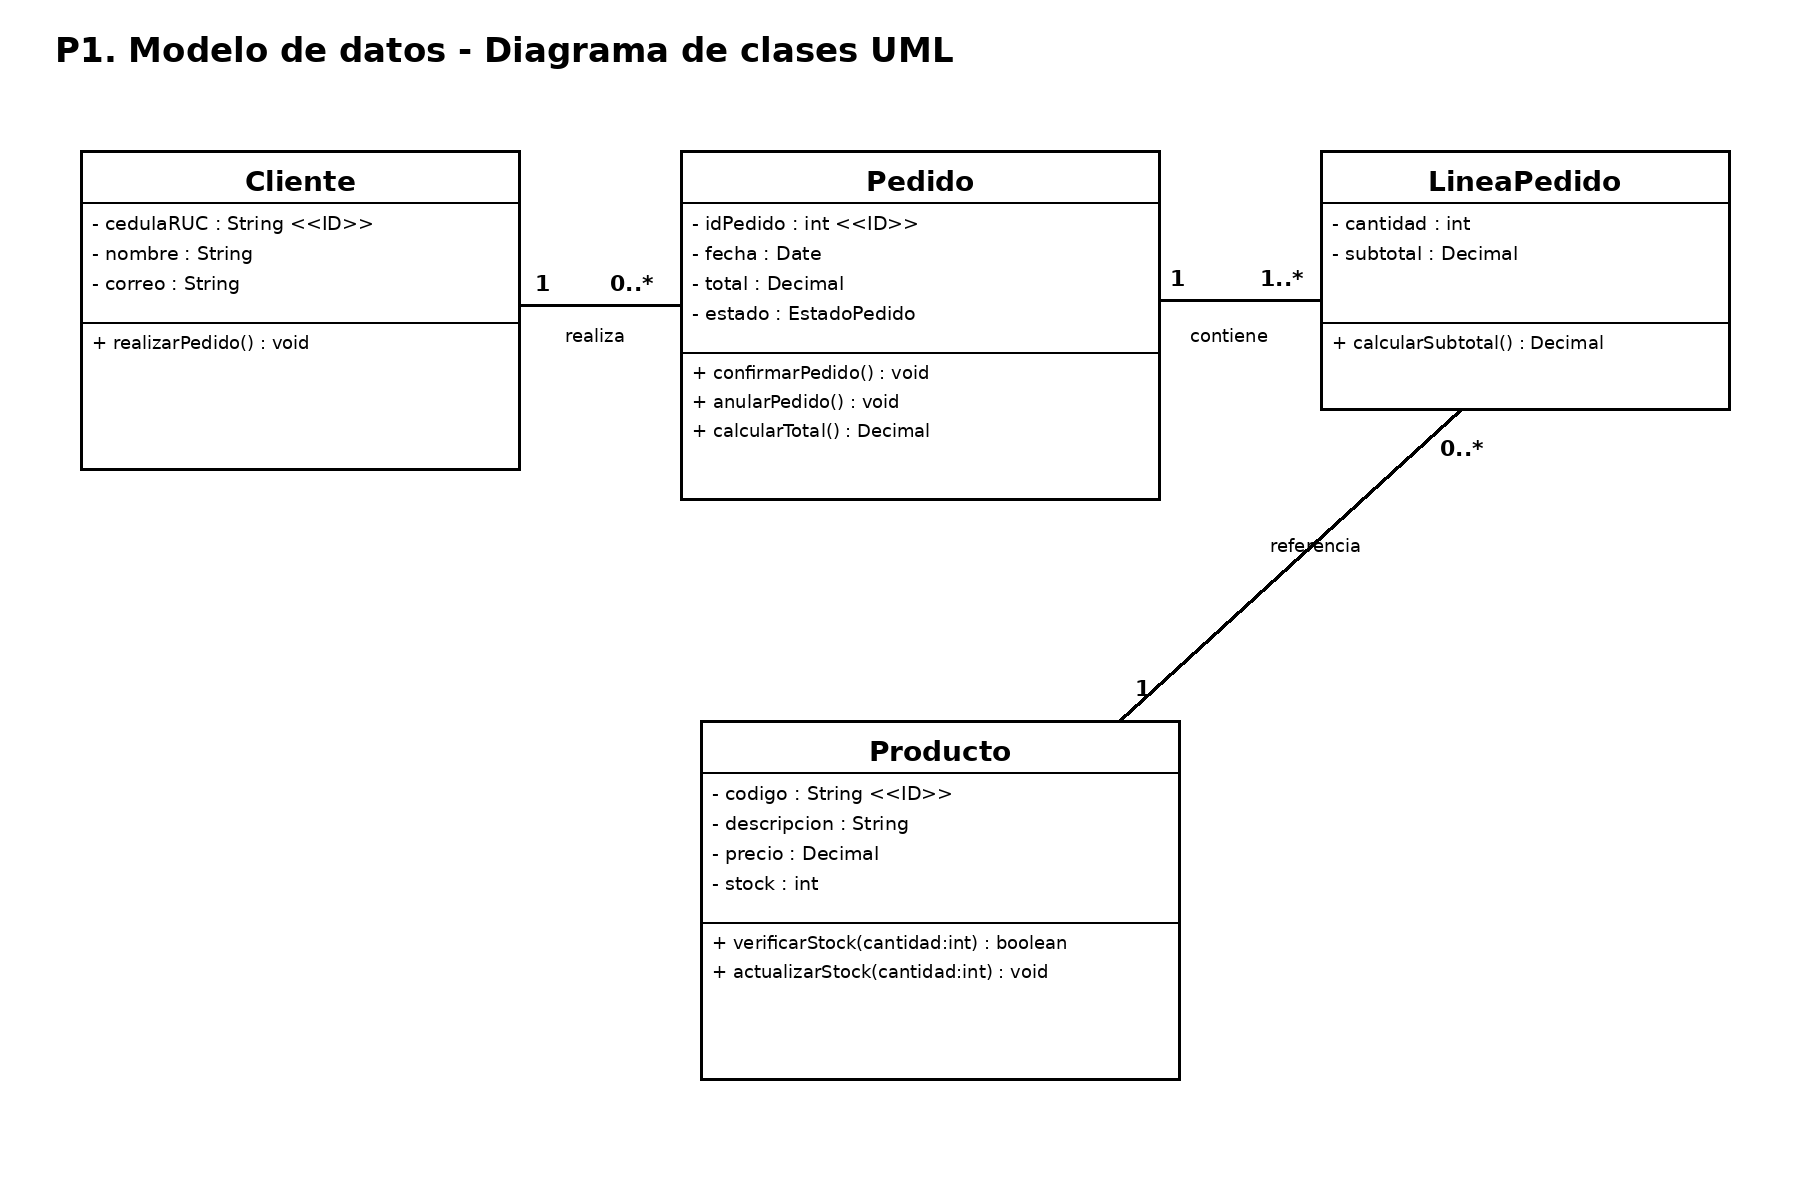
\includegraphics[width=\textwidth]{figuras/p1_diagrama_clases.png}
\caption{Diagrama de clases UML del Sistema de Gestión de Pedidos.}
\end{figure}

Las relaciones representadas son: un Cliente puede realizar de cero a muchos Pedidos; cada Pedido contiene una o más Líneas de pedido; y cada LíneaPedido referencia un Producto.

\section{P2. Modelo funcional - Diagrama de actividades UML}
El proceso \textbf{Registrar pedido} se modeló con dos carriles de responsabilidad, siguiendo el esquema desarrollado a mano: \textbf{Usuario} y \textbf{Base de Datos}. El flujo contiene nodo inicial, verificación de stock, decisión, caminos alternativos y nodos finales.

\begin{figure}[H]
\centering
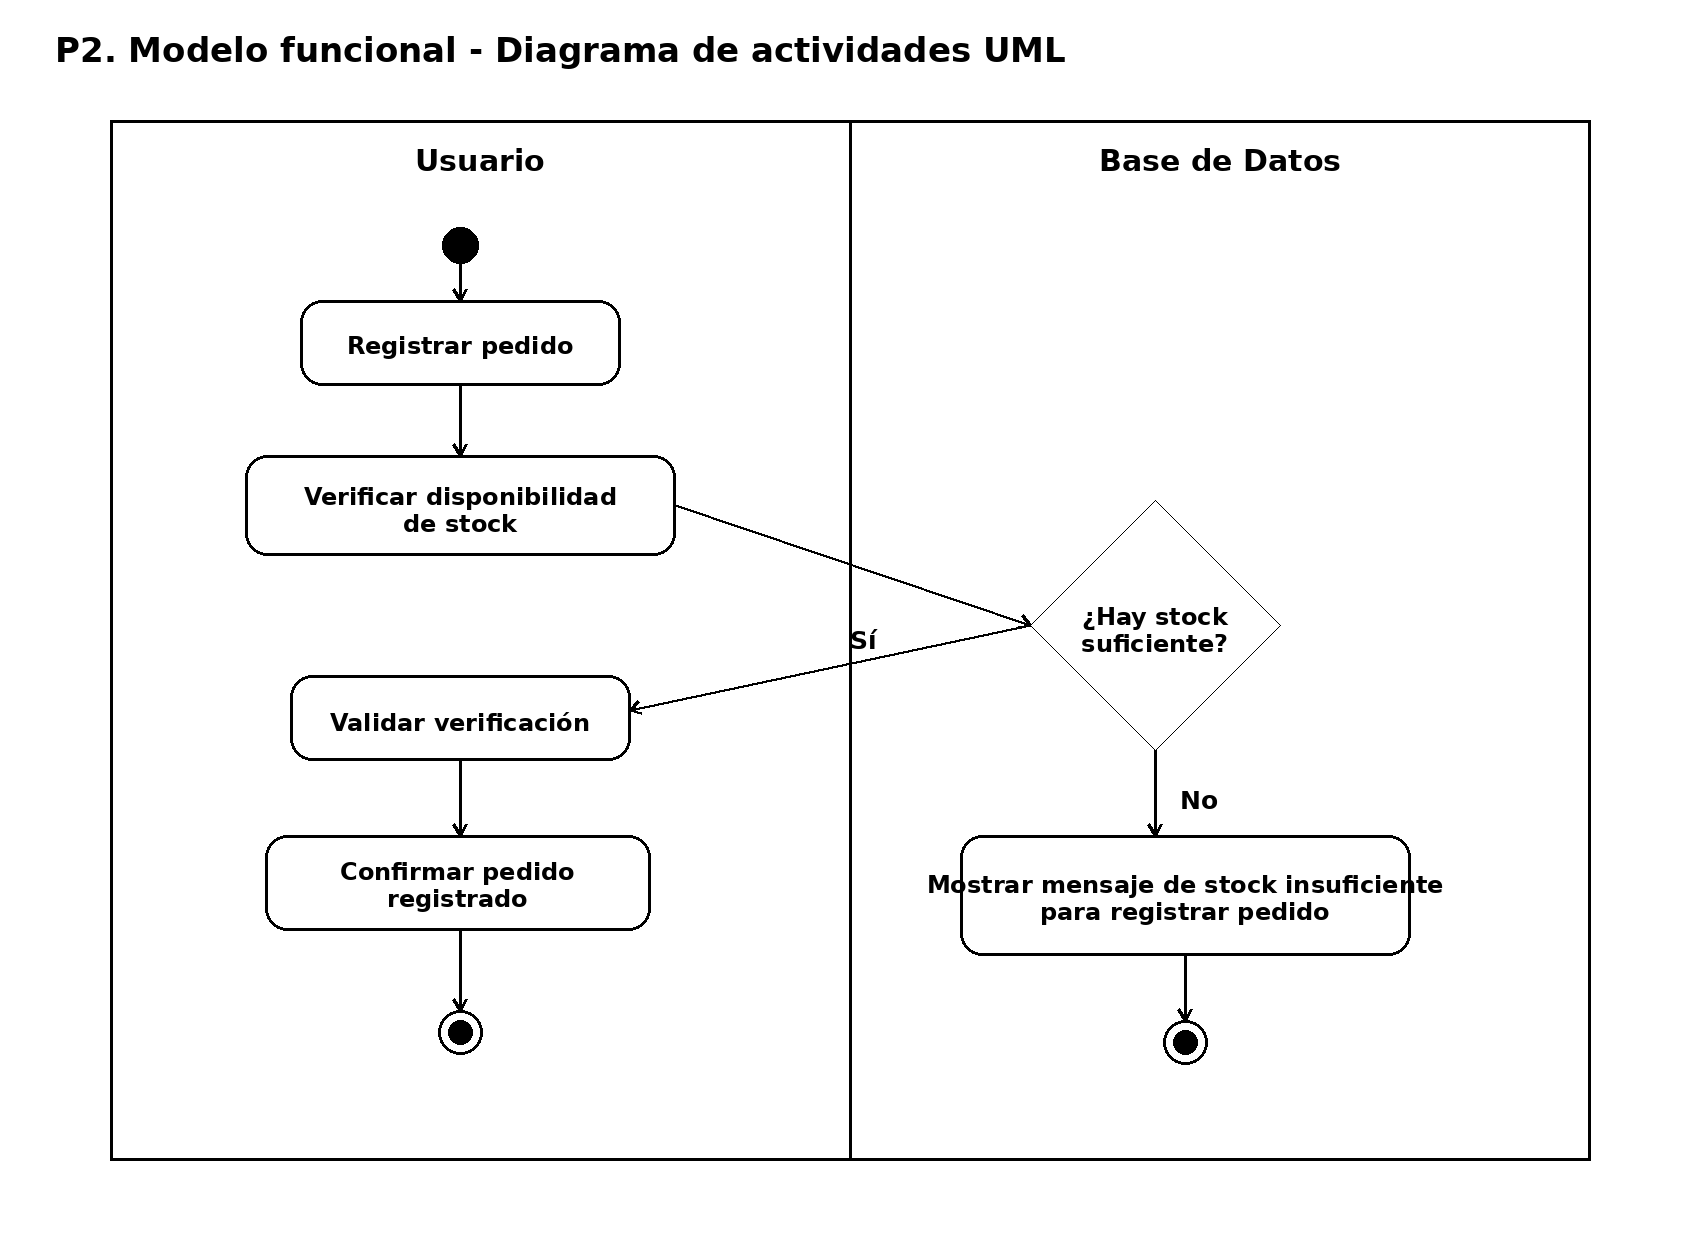
\includegraphics[width=0.96\textwidth]{figuras/p2_diagrama_actividades.png}
\caption{Diagrama de actividades UML del proceso Registrar pedido.}
\end{figure}

\section{P3. Modelo de comportamiento - Máquina de estados UML}
La máquina de estados representa el ciclo de vida del Pedido con estados rectangulares, manteniendo el formato del desarrollo manuscrito. La secuencia principal es Registrado, Confirmado, Enviado y Entregado; adicionalmente se representa el estado Cancelado.

\begin{figure}[H]
\centering
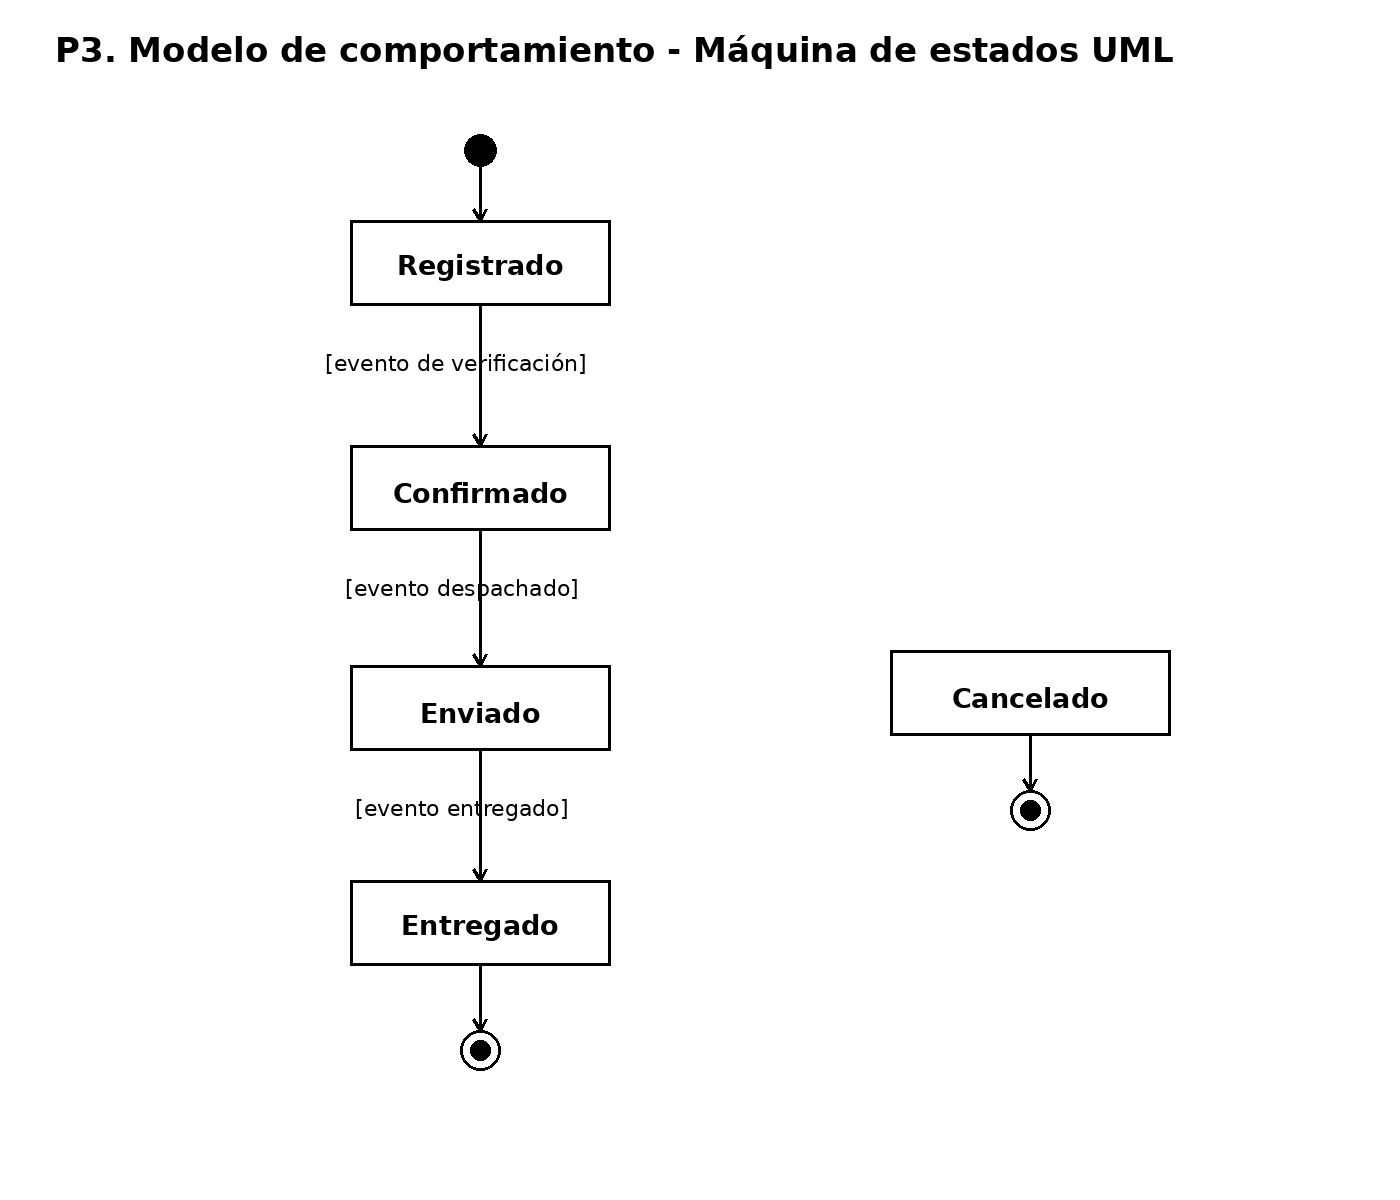
\includegraphics[width=0.88\textwidth]{figuras/p3_maquina_estados.png}
\caption{Máquina de estados UML del ciclo de vida de un Pedido.}
\end{figure}

\section{P4. Consistencia entre las tres perspectivas}
Se elaboró una verificación cruzada entre los eventos del modelo de comportamiento (P3), las funciones del modelo funcional (P2) y las entidades o atributos del modelo de datos (P1).

\begin{center}
\renewcommand{\arraystretch}{1.25}
\small
\begin{tabularx}{\textwidth}{|p{2.7cm}|p{3.6cm}|X|p{2.25cm}|}
\hline
\rowcolor{uteqblue}\color{white}\textbf{Evento de P3} & \color{white}\textbf{Acción / función de P2} & \color{white}\textbf{Entidad o atributo de P1} & \color{white}\textbf{Consistencia} \\
\hline
registrarPedido & Registrar pedido & Pedido.idPedido, Pedido.fecha y Pedido.total & Sí \\
\hline
verificarStock & Verificar disponibilidad de stock & Producto.stock & Sí \\
\hline
confirmarPedido & Confirmar pedido & Pedido.estado & Sí \\
\hline
notificarFaltante & Notificar falta de stock & Producto.stock / LineaPedido.cantidad & Sí \\
\hline
despacharPedido & Despachar pedido & Pedido.estado & Sí \\
\hline
entregarPedido & Entregar pedido & Pedido.estado & Sí \\
\hline
anularPedido & Anular pedido & Pedido.estado & Sí \\
\hline
\end{tabularx}
\end{center}

\subsection*{Inconsistencia detectada y corrección}
\textbf{Defecto detectado:} inicialmente, la clase Pedido del modelo de datos no contenía el atributo \texttt{estado}. Sin embargo, la máquina de estados utiliza los estados Registrado, Confirmado, Enviado, Entregado y Cancelado. Esto producía una inconsistencia entre las perspectivas de datos y comportamiento.

\textbf{Corrección aplicada:} se agregó el atributo \texttt{estado : EstadoPedido} a la clase Pedido. Después de la corrección, los modelos de datos, función y comportamiento mantienen correspondencia entre las operaciones del proceso, los cambios de estado del pedido y los datos almacenados por el sistema.

\section{P5. Especificación de requisitos con esquema de atributos}
Se especificaron dos requisitos funcionales y dos requisitos no funcionales. En los requisitos no funcionales se identifican características de \textbf{ISO/IEC 25010:2023}, junto con métrica y umbral cuantificable.

\subsection{RF-01 - Verificación de stock}
\textbf{Requisito:} El sistema deberá verificar la disponibilidad de stock de cada producto solicitado antes de confirmar un pedido.

\reqtable{RF-01}{Funcional}{Alta}{Propuesto}{Caso Sistema de Gestión de Pedidos}{Alta}{Prueba funcional}

\subsection{RF-02 - Anulación de pedido}
\textbf{Requisito:} El sistema deberá permitir anular un pedido confirmado únicamente cuando este no haya sido entregado.

\reqtable{RF-02}{Funcional}{Alta}{Propuesto}{Caso Sistema de Gestión de Pedidos}{Alta}{Prueba funcional}

\subsection{RNF-01 - Eficiencia de desempeño}
\textbf{Característica ISO/IEC 25010:2023:} Eficiencia de desempeño.

\textbf{Requisito:} El sistema deberá completar el registro y la confirmación de un pedido en un tiempo máximo de 3 segundos, cuando exista stock disponible.

\textbf{Métrica:} tiempo de respuesta del proceso de registro y confirmación.\\
\textbf{Umbral:} $\leq 3$ segundos.

\reqtable{RNF-01}{No funcional}{Media}{Propuesto}{Necesidad de registrar pedidos con rapidez}{Alta}{Prueba de rendimiento}

\subsection{RNF-02 - Seguridad}
\textbf{Característica ISO/IEC 25010:2023:} Seguridad.

\textbf{Requisito:} El sistema deberá impedir el acceso a los datos personales de los clientes a todo usuario que no se encuentre autenticado y autorizado.

\textbf{Métrica:} porcentaje de intentos de acceso no autorizado rechazados.\\
\textbf{Umbral:} 100\% de los intentos no autorizados deberán ser bloqueados.

\reqtable{RNF-02}{No funcional}{Alta}{Propuesto}{Necesidad de proteger los datos personales del cliente}{Alta}{Prueba de seguridad y control de acceso}


\section{P6. Priorización MoSCoW}
Los cuatro requisitos definidos en P5 se priorizaron mediante la técnica \textbf{MoSCoW}, considerando su valor para el funcionamiento del sistema y la viabilidad de implementación.

\begin{center}
\renewcommand{\arraystretch}{1.3}
\small
\begin{tabularx}{\textwidth}{|p{2.2cm}|p{2.6cm}|X|}
\hline
\rowcolor{uteqblue}\color{white}\textbf{Requisito} & \color{white}\textbf{Prioridad MoSCoW} & \color{white}\textbf{Justificación} \\
\hline
RF-01 & Must have & Es indispensable verificar la disponibilidad de stock antes de confirmar un pedido, ya que evita aceptar productos que no se encuentran disponibles. \\
\hline
RF-02 & Must have & La anulación de pedidos es necesaria para gestionar correctamente el ciclo de vida del pedido antes de su entrega. \\
\hline
RNF-01 & Should have & El tiempo de respuesta máximo de 3 segundos mejora la rapidez del registro y confirmación del pedido, pero el sistema puede mantener su funcionalidad principal aunque temporalmente no alcance este nivel de desempeño. \\
\hline
RNF-02 & Must have & La protección de los datos personales del cliente es indispensable; el sistema debe impedir el acceso de usuarios no autenticados o no autorizados. \\
\hline
\end{tabularx}
\end{center}

\textbf{Conclusión de priorización:} RF-01, RF-02 y RNF-02 se clasifican como \textit{Must have} por ser esenciales para la operación y protección de la información. RNF-01 se clasifica como \textit{Should have} debido a que aporta calidad de desempeño sin impedir la operación básica del sistema.

\end{document}
